  \section{Plus de détails sur la physique des neutrinos}\label{app::phyneutrinos}

    \subsection{Le spectre d'énergie des électrons de désintégration \texorpdfstring{$\beta$}{b} : besoin d'une nouvelle particule}\label{sec::neutrino_origin}

      \begin{figure}[htpb]
        \centering
        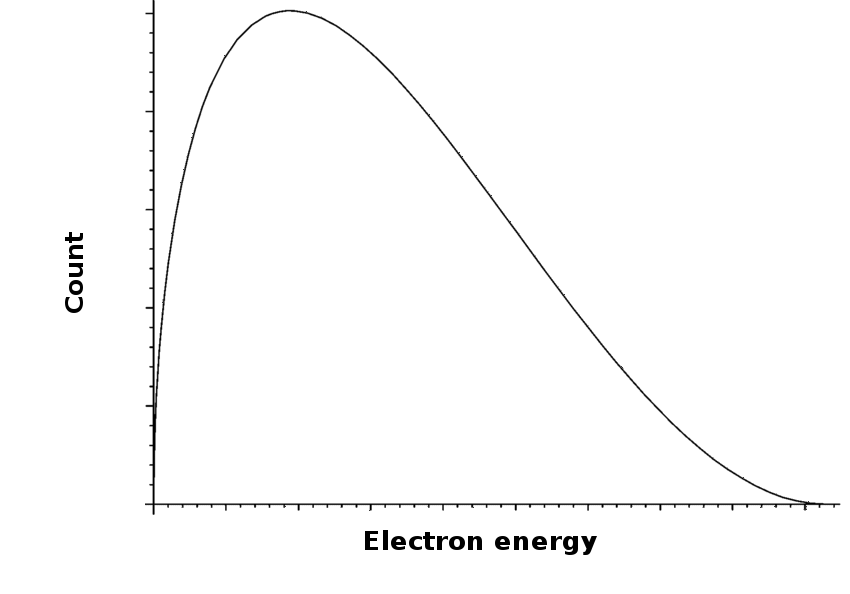
\includegraphics[width=0.6\textwidth,keepaspectratio]{beta_spectrum.png}
        \caption[Spectre de désintégration $\beta$.]{\label{fig::beta_spectrum}Spectre de l'énergie d'un électron émis par une désintégration $\beta$ d'énergie $Q$. Le fait qu'il soit continue entre 0 et $Q$ indique qu'une autre particule est émise en même temps que l'électron.}
      \end{figure}
      La désintégration $\beta$ est la transformation spontanée d'un neutron d'un noyau atomique en proton via l'émission d'un électron et d'un antineutrino électronique. L'énergie émise par une telle désintégration est égale, d'après la formule d'Einstein, à la différence des masses des noyaux avant et après désintégration multipliée par la vitesse de la lumière au carré : 
      \begin{equation}
	    Q = \left[m\left(^A_Z X\right)-m\left(^A_{Z+1} X\right)\right]c^2
      \end{equation}
      Pour un type de noyau $\left(^A_Z X\right)$, cette énergie est constante. La conservation de l'énergie nous dit alors que
      \begin{equation}
	    E_{initial} = E_{final} +E_{e^-}+E_{\anu_e} = E_{final}+Q
      \end{equation}
      où $E_{initial}$ est l'énergie totale du noyau avant désintégration, $E_{final}$ est son énergie après désintégration et $E_{e^-}$ et $E_{\anu_e}$ sont les énergies de l'électron et de l'antineutrino. On a donc $E_{e^-}+E_{\anu_e} = Q$.

      Au moment de la proposition de l'existence du neutrino par Wolfgang Pauli en 1930\cite{Pauli1930}, seul l'électron et le noyau après désintégration étaient détectables, aussi le terme d'énergie $E_{\anu_e}$ était absent de l'équation précédente. Dans ce cas, pour une source radioactive donnée, puisque $Q$ est constante, le spectre en énergie de l'électron aurait due être très piqué atour de $Q$. Or ce n'est pas le cas : ce spectre est continue (voir \autoref{fig::beta_spectrum}) entre 0 et $Q$. En revanche, rajouter à la réaction une particule jusque-là invisible correspond parfaitement à ce spectre, pourvu que la masse de cette particule soit très petite devant $Q$. En effet, si l'antineutrino (et donc le neutrino) avait une masse conséquente, le spectre de l'énergie de l'électron ne pourrait pas atteindre la valeur de $Q$, puisqu'un partie irréductible de $Q$ irait dans la masse du neutrino. C'est d'ailleurs un mesurant avec une très grande précision le spectre de l'énergie des électrons issues de la désintégration du tritium que l'expérience KATRIN\cite{Kleesiek2018} vise à déterminer la masse effective du neutrino électronique avec une précision de \SI{0.2}{\electronvolt\per c\squared}.

    \subsection{Premières observations directes du neutrino}

      Entre les années 30 et 50, la détection du neutrino semblait hors de portée. Il était connu que la probabilité d'interaction de cette particule étant très faible, seule un source très intense de neutrinos pouvait permettre leur observation. Le développement de l'énergie nucléaire dans les années 50 a fourni cette source : les réactions de fission sont accompagnées de l'émission d'antineutrinos électroniques en très grande quantité.

      Entre 1952 et 1953, Frederick Reines et Clyde Cowan construisent un détecteur dont le matériau de réaction est simplement de l'eau. Un antineutrino incident interagissant avec un proton produit une réaction $\beta$ inverse produisant un neutron et un positron, se dernier s'annihilant rapidement avec un électron pour donner deux photons. Le signal attendu est alors un dépôt d'énergie électromagnétique suivie par l'interaction d'un neutron avec l'eau caractérisée par l'émission d'un troisième photon, après absorption du neutron par un noyau de chlorure de cadmium, un bon absorbeur de neutron que Reines et Cowan avaient dissous dans l'eau. La détection des photons s'effectuait dans une couche de scintillateur liquide munie de tubes photomultiplicateurs entourant les deux cuves de détection. Le volume d'eau total était de $\SI{200}{\liter}$ où étaient dissous $\SI{40}{\kilogram}$ de chlorure de cadmium. Le flux de d'antineutrinos attendu du réacteur était de l'ordre de $\SI{e13}{\anu_e\second^{-1}\centi\meter^{-2}}$.

      La première tentative de détection du neutrino fut faite auprès du réacteur nucléaire de Hanford dans l'état de Washington, sans donner de résultat concluant. La seconde tentative, proche du réacteur de Savannah River en Caroline du Sud, détecta un signal de \SI{2.88}{\text{coups}\per\hour}\cite{Cowan1956} pour 1371 heures de prises de données, 20 fois supérieur au bruit de fond attendu, démontrant finalement l'existence d'une particule légère, et particulièrement peu réactive, dans la réaction $\beta$. La section efficace mesurée de  \SI{6.3e-44}{\centi\meter\squared} était compatible avec la valeur tirée des mesures de désintégration du neutron de Robson\cite{Robson1951}, de \SI{6e-44}{\centi\meter\squared}.

      Aujourd'hui, les expériences cherchant à détecter des neutrinos sont conçues de manière semblable à l'expérience de Reines et Cowan : un volume important, contenant un milieu dense,  afin d'offrir un maximum de protons cibles sur lesquels les neutrinos  peuvent interagir, une source de neutrinos intense et un temps d'exposition long. La réduction du bruit de fond est essentielle dans une telle expérience : lors de leur seconde tentative, Reines et Cowan ont en effet placé leur détecteur sous terre. Ceci leur a permit de réduire grandement le taux de rayons cosmiques arrivant dans leur détecteur. En effet, ces derniers étaient susceptibles de créer des signaux semblables à celui attendu pour une interaction neutrino. Cette technique est encore largement employée aujourd'hui dans les expériences détectant des neutrinos.

      L'eau est encore utilisée aujourd'hui pour détecter des neutrinos, par exemple dans l'expérience Super-Kamiokande\cite{Fukuda1998}, mais des détecteurs solides ont également vu le jour comme dans les expériences \gls{nova}\cite{Adamson2016} et \gls{opera}\cite{Agafonova2018}. Une des techniques les plus récentes utilise comme cible des gaz nobles liquéfiés, plus dense que l'eau, notamment l'argon dans l'expérience prototype \gls{icarus}\cite{Amerio2004} et la future expérience \gls{dune}\cite{Acciarri2016a}. 

      Les réacteurs nucléaires sont encore beaucoup utilisés dans les expériences de neutrinos, par exemple par Double Chooz\cite{Crespo-Anadon2014}, Daya Bay\cite{An2014}, RENO\cite{Collaboration2010} et la future JUNO\cite{An2015}. Les faisceaux de neutrinos créés artificiellement, plus contrôlables que les réacteurs, ont été inventés dans les années 60. L'expérience \gls{t2k}\cite{Abe2018} détecte des neutrino issus d'un faisceau, et ce sera le cas également de l'expérience \gls{dune}\cite{Strait2016}. Des sources naturelles existent aussi : le soleil fourni un important flux de neutrinos, étudiés par des expériences comme \gls{sno}\cite{Aharmim2013}. Cette dernière, avec Super-Kamiokande\cite{Fukuda1998} qui détecte des neutrinos produits par des rayons cosmiques dans l'atmosphère, a permis de mettre en évidence le phénomène d'oscillation des neutrinos dont nous parlerons en détail dans la prochaine section. Les deux expériences ont reçu le prix Nobel de physique en 2015. Enfin, les neutrinos issus de supernovae peuvent également être détectés, pourvu qu'une supernovae explose durant une prise de données d'une expérience. C'est arrivé une seule fois en 1987, où 20 événements neutrinos ont été détectés par les détecteur IMB et Kamikande II\cite{Hirata1987}.

    \subsection{Les 3 familles de neutrinos}

      \begin{figure}[htpb]
        \centering
        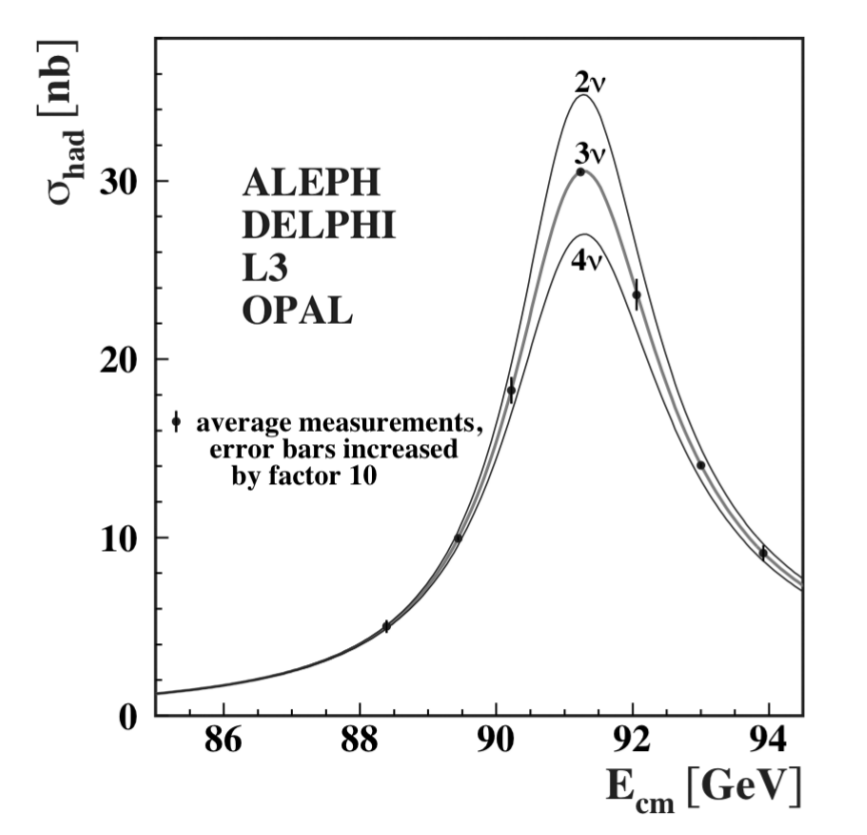
\includegraphics[width=0.6\textwidth,keepaspectratio]{three_neutrinos.png}
        \caption[Spectre de désintégration $\beta$.]{\label{fig::three_neutrinos}Mesure de la section efficace de production de hadron en fonction de l'énergie dans le centre de masse au LEP autour de la masse du boson $Z^0$. Résultats combinés des quatre expériences. Les courbes représentent les prédictions théoriques pour un nombre de saveurs de neutrinos actifs de 2, 3 et 4, les points sont les résultats de mesures, qui montre qu'il y a 3 familles de neutrinos actifs. Les incertitudes sont agrandies d'un facteur 10. Graphique tiré de \cite{Mele2015}.}
      \end{figure}
      Le muon, découvert en 1937 par Street et Stevenson\cite{Street1937}, ne diffère de l'électron que part sa masse. Ce dernier étant (théoriquement, à l'époque) produit avec un neutrino dans les désintégrations $\beta$, il paraissait plausible que le muon puisse également être lié au neutrino d'une manière ou d'une autre.  Le spectre en énergie de l'électron produit par la désintégration du muon, mesuré par Leighton, Anderson et Seriff en 1949\cite{Leighton1949}, est continu. Un raisonnement identique à celui de Pauli de 1930 montre que le muon doit se désintégrer en trois particules : un électron et deux neutrinos. Il fallut cependant attendre 1962 et les expériences sur faisceau de neutrinos de Lederman, Steinberger et Schwartz\cite{Danby1962} pour détecter le neutrino muonique et définitivement montrer qu'il était différent du neutrino électronique : les neutrinos du faisceau, produits par la désintégration de muons, ne créaient que des muons dans le détecteur et aucun électron\footnote{Proche de la source, la probabilité  de changement de saveur lié au phénomène des oscillations des neutrinos est trop faible pour induire une composante autre que du neutrino muonique.}.

      La découverte du troisième lepton, le $\tau$, en 1975 par Perl\cite{Perl1975} n'a pas tardé à être suivi par la prédiction d'un troisième neutrino associé, le neutrino tauique. Ce dernier fut détecté en 2000 par l'expérience \gls{donut}\cite{Collaboration2000}. Un faisceau de neutrinos issu du Fermilab, contenant toutes les saveurs possibles de neutrino, interagit avec un détecteur capable d'identifier les produits de réactions. Ce dernier a observé 4 événements neutrinos ayant créé un $\tau$.

      Les trois familles de quarks up--down, strange--charmed et top--bottom et les trois familles de leptons, l'électron et son neutrino, le muon et son neutrino et le tau et son neutrino, avaient alors été observées. Les quatre expériences du LEP, en étudiant la production de hadron à une énergie dans le centre de masse autour de la masse du boson $Z^0$, un des vecteurs de l'interaction faible, avait montré en 1989 qu'il ne pouvait pas exister plus de 3 saveurs de neutrinos légers sensibles à l'interaction faible\cite{DeCamp1989} (un graphique de cette étude est présenté en \autoref{fig::three_neutrinos}). Tous les neutrinos que nos instruments permettent de voir avaient alors été observés.

    \subsection{Les symétries discrètes du modèle standard}\label{sec::CP}

      Un des principes fondamentaux du modèle standard, au même titre que la conservation de l'énergie, est que toute prédiction de ce dernier doit être identique après conjugaison Charge-Parité-Temps (CPT). Autrement dit, après avoir inversé la charge et les coordonnées spatio-temporelles.

      La conjugaison de charge inverse les charges -- électrique, isospin faible et couleur -- d'une particule. Un électron, par exemple, est transformé en positron, et de manière plus générale n'importe quelle particule chargée en son antiparticule. La transformation de parité consiste à prendre un système ou processus physique  et à le regarder dans un miroir. Autrement dit, remplacer toutes les coordonnées d'espace par leur opposées : $\Vec{r}\to-\Vec{r}$. Si la parité laisse le système ou processus inchangé, ce dernier est dit pair. Si au contraire il devient son opposé, il est dit impair. Un bon exemple de grandeur impaire est l'impulsion : $\Vec{p}(-\Vec{r}) = m(-\dot{\Vec{r}}) = -\Vec{p}(\Vec{r})$. À l'inverse, une grandeur paire est le moment cinétique : $\Vec{L}(-\Vec{r}) = -\Vec{r}\times -\Vec{p} = \Vec{L}(\Vec{r})$. L'extension à la mécanique quantique consiste à dire qu'un état est pair(impair) si il est état propre de l'opérateur de conjugaison de parité $\hat{P}$, qui inverse les coordonnées d'espace, avec une valeur propre de $+1(-1)$. Dans le modèle standard, une particule de spin $1/2$ est représentée par un spineur de Dirac $\psi(x,t)$, qui est composée de deux spineurs de Weyl :
      \begin{equation}
        \psi(x,t)=\left(\begin{matrix} u_R(x,t) \\ u_L(x,t)\end{matrix}\right)
      \end{equation}
      où $R$ et $L$ signifie "droite"(right) et "gauche"(left). Ils sont caractérisés par la manière dont un boost de Lorentz agit sur eux : ils acquièrent tous deux un facteur de phase, mais ces deux phases sont de signe opposé. Une transformation de parité transforme $u_R$ en $u_L$ et inversement. La dernière caractéristique importante d'un spineur de Weyl est qu'il est de masse nulle, alors qu'un spineur de Dirac peut avoir une masse $m_D$ : le lagrangien libre de Dirac, qui décrit comment évolue un spineur de Dirac sans interaction, autorise un terme de masse de la forme
      \begin{equation}\label{eq::dirac_mass}
        -m_D(\overline{u}_R u_L + \overline{u}_L u_R)
      \end{equation}
      où $\overline{u}_{R/L}$ est le conjugué de Dirac de $u_{R/L}$. Autrement dit, un fermion massif doit nécessairement avoir ses deux composantes gauche et droite non nulles. En revanche, il est possible qu'un fermion de masse nulle n'existe que dans un état de chiralité, gauche ou droite, auquel cas il peut être décrit par un spineur de Weyl $u_{R/L}$ seul. 

      La transformation de temps revient à inverser la flèche du temps et donc à regarder un processus dans l'autre sens. Par exemple, l'annihilation d'un électron avec un positron pour donner un photon devient l'émission d'une paire électron-positron par un photon.

      \begin{figure}[htpb]
        \centering
        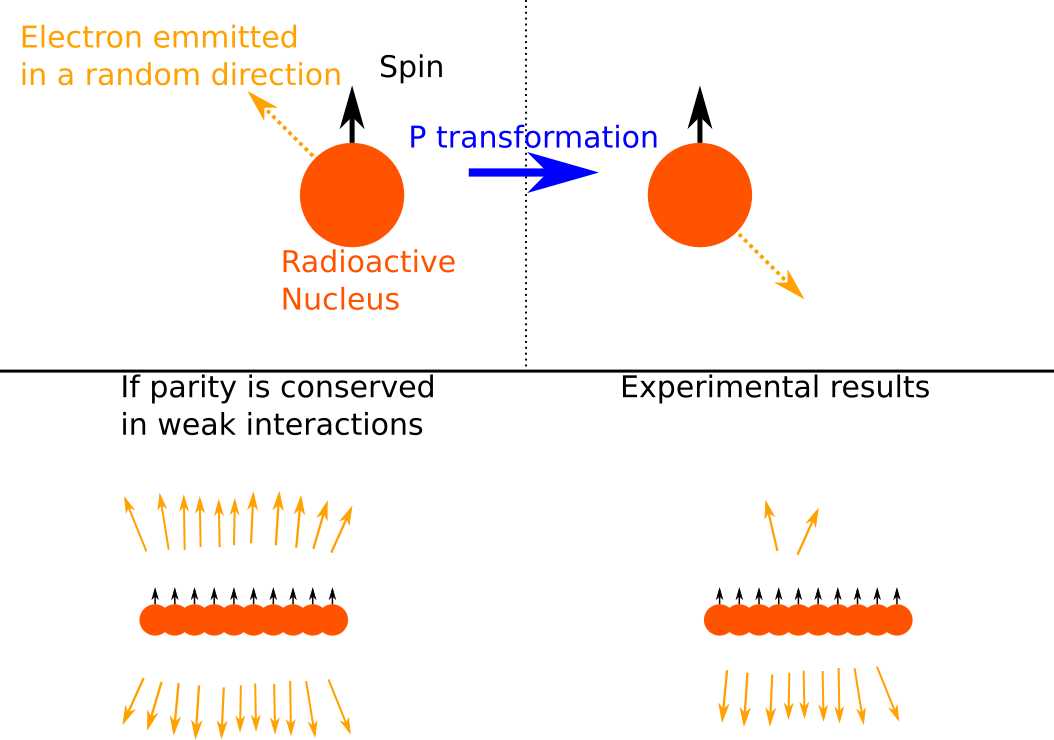
\includegraphics[width=0.7\textwidth,keepaspectratio]{wu2.png}
        \caption[Principe de l'expérience réalisée par C.S. Wu en 1957.]{\label{fig::wu}Principe de l'expérience réalisée par C.S. Wu en 1957 : un groupe de noyaux radioactif dont les spins sont tous orientés dans la même direction doivent émettre des électrons de manière isotrope si la conjugaison de partié est une symétrie de l'interaction faible. Il a été observer que les électrons étaient en majorité émis dans la direction opposée au spin, démontrant la violation de la symétrie $P$ par l'interaction faible.}
      \end{figure}

      Jusqu'en 1956, tous les processus physiques observés étaient invariants par transformation de parité, et cette dernière était considéré comme une symétrie de la nature. Mais cette même année, Tsung Dao Lee et Chen Ning Yang\cite{Lee1956} se rendent compte que, bien que bon nombre d'expériences montrent que les interactions forte et électromagnétique sont en effet symétriques par transformation de parité, aucune n'a étudié la question pour l'interaction faible. Ils proposent alors plusieurs méthodes expérimentales permettant de tester la conservation de la parité de l'interaction faible. L'une de ces expériences est réalisée entre 1956 et 1957 par Chieng-Shiung Wu. Elle consiste à étudier la distribution spatiale des électrons émis par des noyaux radioactifs $\beta$ avec des spins alignés. La \autoref{fig::wu} schématise le signal recherché : le spin est invariant par transformation de parité alors que l'impulsion change de signe. L'image miroir d'un noyau émettant un électron dans la même direction que son spin est donc le même noyau émettant cet électron dans la direction opposée au spin. Le processus miroir est donc différent du processus initial et donc, pour que la désintégration $\beta$ soit symétrique par rapport à la transformation de parité, il faut qu'un ensemble de noyaux radioactifs dont les spins sont alignés émettent en moyenne autant d'électrons dans la direction de leur spin que dans la direction opposée. Or, l'expérience montre que ce n'est pas le cas : l'électron est en écrasante majorité émis dans la direction opposée au spin\cite{Wu1957}. L'interaction faible viole donc la symétrie $P$. Tsung Dao Lee et Chen Ning Yang reçoivent le prix Nobel en 1957 pour ces travaux.

      L'expérience de C.S Wu, et plus tard celle de Goldhaber\cite{Goldhaber1958} en 1957, ont montré que l'interaction faible n'agit que sur la composante de chiralité gauche d'un spineur de Dirac, autrement dit la composante $\psi_L(x,t)=\left(\begin{matrix}0 \\ u_L(x,t)\end{matrix}\right)$. C'est pour cela qu'elle ne conserve pas la symétrie P. La masse du neutrino étant alors considérée comme nulle, il était naturel d'utiliser un spineur de Weyl de chiralité gauche pour décrire le neutrino, et un spineur de Weyl de chiralité droite pour décrire l'antineutrino.

      Puisque le neutrino est de charge nulle, une conjugaison de charge ne saurait le changer en son antineutrino. En effet, ce dernier n'existe que dans un état de chiralité droite, il faut donc également appliquer un transformation de parité. On peut donc se poser la question suivante : la transformation CP est-elle une symétrie du modèle standard? Si c'est le cas, les neutrinos et les antineutrinos doivent se comporter de la même manière. De manière générale, toute la matière décrite par le modèle standard se comporterait alors comme l'antimatière. Mais ceci soulève alors une question encore plus fondamentale : pourquoi n'y a-t-il plus d'antimatière dans l'univers? En effet, les théories actuelles du big bang\cite{Canetti2012} montrent qu' il devait y avoir autant de matière que d'antimatière à la création de l'univers. Matière et antimatière s'annihilent si elles se rencontrent, l'univers devrait être composé essentiellement de vide et de photons. Or ce n'est pas le cas : l'antimatière a disparu et la matière est restée. Le phénomène, appelé baryogenèse, responsable de cette asymétrie est encore mal connu, mais le fait que l'antimatière ne se comporte pas tout à fait comme la matière est nécessaire\cite{Sakharov1991}

      Il a été expérimentalement prouvé que la symétrie CP n'est pas conservée dans le secteur des quark\cite{Collaboration2006,Charles2004,Kobayashi1973}: la matrice de mélange CKM contient une phase complexe introduisant un comportement légèrement différent entre les quarks et les antiquarks. Mais la violation de CP dans ce secteur n'est pas suffisante pour expliquer la baryogenèse\cite{Riotto1998}. En revanche, l'observation d'une violation de CP dans le secteur des leptons peut l'expliquer\cite{Davidson2008}. Comme nous le montrerons plus loin, le phénomène d'oscillation des neutrinos introduit également une phase complexe pouvant créer une différence de comportement entre matière et antimatière.

    \subsection{La masse du neutrino : Dirac ou Majorana?}\label{sec::dirac_majorana}

      \begin{activitybox}[label=box::mass_term]{Comment construire un terme de masse dans un lagrangien?}
        Un terme de masse dans un lagrangien doit respecter les critères suivants :
        \begin{itemize}
          \item[$\bullet$] Être invariant de Lorentz (i.e respecter la relativité restreinte).
          \item[$\bullet$] Avoir la dimension d'une énergie (le lagrangien est une énergie).
          \item[$\bullet$] Il doit faire intervenir la champ de la particule dont il est la masse.
          \item[$\bullet$] Il doit être réel, donc faire intervenir le champ et son conjugué complexe.
        \end{itemize}
        Le terme le plus simple respectant tous ces critères est, pour un fermion décrit par un champ $\psi$, de la forme $-m\bar{\psi}\psi$.
      \end{activitybox}

      Nous avons vu dans la section précédente qu'un neutrino sans masse peut être décrit par un spineur de Weyl. Depuis la mise en évidence de la masse des neutrinos par le phénomène d'oscillation, il est clair que cette description est insuffisante, un spineur de Weyl ne pouvant pas avoir de terme de masse dans un lagrangien de Dirac. L'extension la plus simple consiste à considérer le neutrino comme un spineur de Dirac et de lui adjoindre le terme de masse \eqref{eq::dirac_mass} (voir l'encadré \ref{box::mass_term} pour une explication sur comment créer un terme de masse). Dans ce cas, le neutrino aura une composante de chiralité droite non nulle, qui n'interagit avec aucune interaction du modèle standard. Il peut interagir par gravitation, mais cette dernière est bien trop faible pour être détectable à l'échelle de la physique des particules. 

      Il existe une autre possibilité pour un terme de masse du neutrino: par son absence de charge, le neutrino peut également être décrit par un fermion de Majorana, dont le terme de masse est très différent de celui d'un fermion de Dirac. Un spineur de Majorana a la particularité qu'il est sa propre antiparticule. Dans le modèle standard, seul le neutrino peut être décrit par un spineur de Majorana. En effet, les autres fermions ayant une charge électrique, ils ne peuvent pas être leur propre antiparticule qui doit être de charge opposée. Dans ce cas là, un nouvel état de chiralité droite n'est pas nécessaire, et donc aucun neutrino stérile n'est introduit (une discussion plus détaillée ce trouve ici\cite{Petcov2013}).

      Nous avons écrit en section précédente le terme de masse d'un spineur de Dirac. Pour un neutrino dans un état propre de l'hamiltonien $\nu_i=\nu_R+\nu_L$, nous avons donc : 
      \begin{equation}
	    -m_D\anu_R \nu_L + \text{conjugué complexe}
      \end{equation}
      Ce terme de masse est créé, comme pour les autres fermions, par interaction du champ de neutrino avec le champ de Higgs après brisure de symétrie via un couplage de Yukawa. Il n'implique pas forcément de physique au-delà du modèle standard.

      Un terme de masse de Majorana quant à lui est de la forme
      \begin{equation}\label{eq::majorana_mass}
        -\frac{1}{2}m_M\anu_L^T C \nu_L + \text{conjugué complexe}
      \end{equation}
      où $C$ est la matrice de conjugaison de charge. Comme l'explique B. Kayser dans \cite{Kayser2009}, un tel terme ne peut pas être créé par un couplage de Yukawa, mais par une interaction plus complexe avec le champ de Higgs qui n'est pas décrite par le modèle standard. Un terme de masse de Majorana pourrait expliquer la petitesse des masses des neutrinos par le mécanisme dit de see-saw , qui prédit l'existence de neutrinos ultra-lourds (\numprint{e9}--\SI{e15}{\giga\electronvolt}). Si la symétrie CP n'est pas conservée, ces derniers se seraient désintégrés à l'origine de l'univers en produisant un peu plus de matière que d'antimatière (voir l'article deB. Kayser\cite{Kayser2005}).

      Les différences de comportement entre neutrino de Dirac et de Majorana sont difficiles à observer. La plus recherchée en ce moment est la désintégration double-beta sans émission de neutrino, qui n'est possible que si le neutrino est sa propre antiparticule. Aucun résultat concluant n'a été observé à ce jour\cite{Dolinski2019}.